
\preClass{Complex Numbers}

\begin{problem}
\item Expand each of the expressions below. (You will need to ``FOIL''
  the expressions.) In each case treat the parameter $i$ as a
  constant number.

  \begin{subproblem}
  \item $(4+3i)*(5-6i)$

      \iftoggle{solutions}{%

        \begin{eqnarray*}
          20 + 15 i - 24 i - 18 i^2 & = & 20 - 9i - 18 i^2.
        \end{eqnarray*}
        
      }

    \vfill

  \item $(2+i)(10+4i)$

      \iftoggle{solutions}{%

        \begin{eqnarray*}
          10 + 10i + 8i + 4i^2 & = & 10 + 18i + 4i^2.
        \end{eqnarray*}
        
      }

    \vfill
      
  \item $(2-i)(2+i)$

      \iftoggle{solutions}{%

        \begin{eqnarray*}
          4 - 2i + 2i  - i^2 & = & 4 - i^2.
        \end{eqnarray*}
        
      }

    \vfill

  \item $(6+3i)(6-3i)$

      \iftoggle{solutions}{%

        \begin{eqnarray*}
          36 + 18i - 18i - 9i^2 & = & 36 - 9 i^2.
        \end{eqnarray*}
        
      }

    \vfill

  \end{subproblem}
\end{problem}



  \actTitle{Complex Numbers}
  \begin{problem}
  \item Find the solution to the following differential equation:
    \begin{eqnarray*}
      y' & = & k y, \\
      y(0) & = & 1,
    \end{eqnarray*}
    where $k$ is a constant.

    \iftoggle{solutions}{%

      \begin{eqnarray*}
        y(t) & = & C e^{kt}, \\
        y(0) & = & C e^0, \\
        1 & = & C, \\
        y(t) & = & e^{kt}.
      \end{eqnarray*}
        
    }

    \vfill

  \item Replace the constant ``k'' with a constant called ``$i$'' and
    find the solution to the following differential equation:
    \begin{eqnarray*}
      y' & = & i y, \\
      y(0) & = & 1.
    \end{eqnarray*}
    \label{problem:firstLookEulerFormula}

      \iftoggle{solutions}{%

        \begin{eqnarray*}
          y(t) & = & C e^{it}, \\
          y(0) & = & C e^0, \\
          1 & = & C, \\
          y(t) & = & e^{it}.
        \end{eqnarray*}
        
      }

    \vfill


    \clearpage
  \item Define the constant ``i'' to be $\sqrt{-1}$. Find each of the
    following values:

    \begin{subproblem}
      \item $i^2$

      \iftoggle{solutions}{%

        \begin{eqnarray*}
          i^2 & = & -1.
        \end{eqnarray*}
        
      }

        \vfill
      \item $i^3$

      \iftoggle{solutions}{%

        \begin{eqnarray*}
          i^3 & = & -i.
        \end{eqnarray*}
        
      }

        \vfill
      \item $i*(1+i)$

      \iftoggle{solutions}{%

        \begin{eqnarray*}
          i*(1+i) & = & i + i^2, \\
          & = & i-1.
        \end{eqnarray*}
        
      }

        \vfill
    \end{subproblem}

  \end{problem}


  \actTitle{Complex Numbers}
  \begin{problem}

  \item Define $y(t)$ to be the following function:
    \begin{eqnarray*}
      y(t) & = & \cos(t) + i \sin(t).
    \end{eqnarray*}
    Answer each of the following questions. Keep in mind that $i$ is a
    constant.

    \begin{subproblem}
      \item Determine the derivative of $y(t)$. 

        \iftoggle{solutions}{%

          \begin{eqnarray*}
            y'(t) & = & -\sin(t) + i \cos(t).
          \end{eqnarray*}
        
        }

        \vfill

      \item Determine and simplify $i*y(t)$.

        \iftoggle{solutions}{%

          \begin{eqnarray*}
            i\cdot y(t) & = & i\cos(t) + i^2 \sin(t), \\
            & = & i\cos(t) - \sin(t).
          \end{eqnarray*}
        
        }

        \vfill

        \clearpage

      \item Show that $y(t)$ is a solution to the following
        differential equation:
        \begin{eqnarray*}
          y' & = & i y, \\
          y(0) & = & 1.
        \end{eqnarray*}

        \iftoggle{solutions}{%

          \begin{eqnarray*}
            y'(t) & = & -\sin(t) + i \cos(t), \\
            i \cdot y & = & -\sin(t) + i \cos(t), \\
            y(0) & = & \cos(0) + i \sin(0), \\
            & = & 1.
          \end{eqnarray*}
          It is a solution to the differential equation.

        
        }

        \vfill

      \item Recall the solution of the previous differential equation
        given in problem \ref{problem:firstLookEulerFormula}, page
        \pageref{problem:firstLookEulerFormula}. (Write it down here.)

        \iftoggle{solutions}{%

          \begin{eqnarray*}
            y & = & e^{it}.
          \end{eqnarray*}
        
        }{\vspace{4em}}

      \item What is the relationship between that solution and the
        function $y(t)$?

        \iftoggle{solutions}{%

          They are the same.
        
        }

        \vfill
        

    \end{subproblem}

    \clearpage

  \item Express the variable $x$ in terms of $r$ and $\theta$. Do the
    same for $y$. Determine how to find $r$ and $\theta$ given $x$ and
    $y$. 

    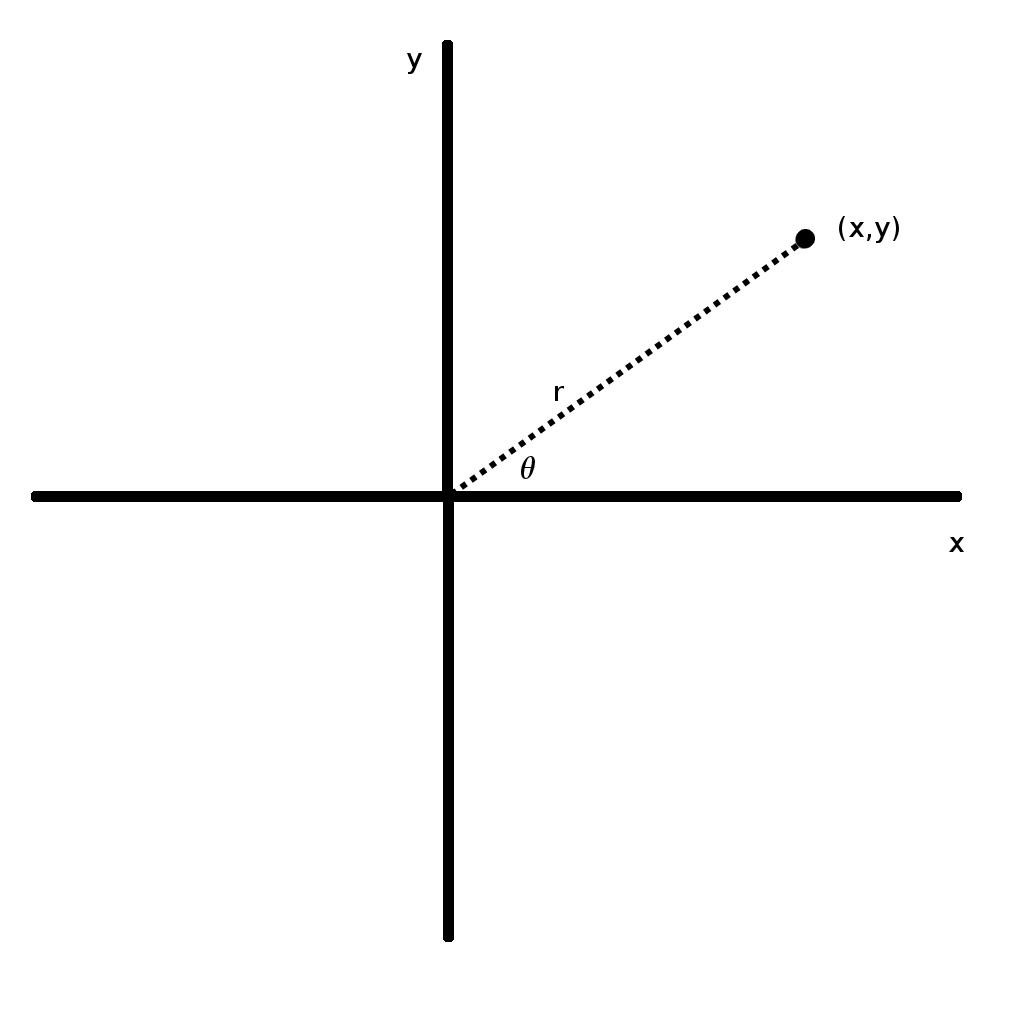
\includegraphics[height=12cm]{img/polar}

    \iftoggle{solutions}{%

      Express $x$ and $y$ in terms of $r$ and $\theta$:
      \begin{eqnarray*}
        x & = & r\cos(\theta), \\
        y & = & r\sin(\theta).
      \end{eqnarray*}

      Express $r$ and $\theta$ in terms of $x$ and $y$:
      \begin{eqnarray*}
        r & = & \sqrt{x^2+y^2}, \\
        \tan(\theta) & = & \frac{y}{x}.
      \end{eqnarray*}
        
    }

    \vfill


  \end{problem}
